\documentclass[../cours_tle.tex]{subfiles}
\begin{document}
\setcounter{chapter}{33}
\chapter{Graphes, chemins et matrices d’adjacence}
\label{ch:34}
\begin{objectif}
Mathématiques expertes. Modéliser des relations et compter des parcours. Prérequis : dénombrement et multiplication matricielle.
\end{objectif}
\section{Vocabulaire et conventions}
Un graphe possède des sommets et des arêtes reliant certains sommets. Sauf indication contraire, les graphes non orientés étudiés ici sont simples : sans boucle ni arêtes multiples.
Son ordre est le nombre de sommets ; le degré d'un sommet compte les arêtes incidentes. Deux sommets sont adjacents si une arête les relie.
Le graphe complet $K_n$ relie chaque paire de sommets distincts : il possède $\binom n2$ arêtes et chaque degré vaut $n-1$.
Un parcours de longueur $k$ utilise successivement $k$ arêtes, avec répétitions autorisées. Cette convention de « chemin » est celle utilisée dans les puissances de matrices ; un chemin simple, sans sommet répété, est une notion plus restrictive.
Un graphe est connexe si chaque paire de sommets est reliée par un parcours.
\section{Le lemme des poignées de main}
\begin{propriete}
La somme des degrés d'un graphe simple non orienté vaut deux fois le nombre d'arêtes. Le nombre de sommets de degré impair est pair.
\end{propriete}
\begin{demonstration}
Chaque arête contribue $1$ au degré de chacune de ses deux extrémités. La somme est donc paire. Les degrés pairs ne changent pas sa parité ; le nombre de termes impairs doit être pair.
\end{demonstration}
\begin{center}
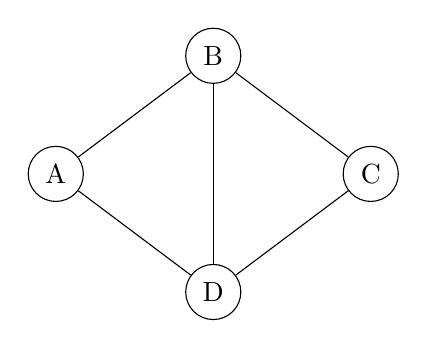
\begin{tikzpicture}[every node/.style={circle,draw,minimum size=7mm}]
\node(A)at(0,0){A};\node(B)at(2,1.5){B};\node(C)at(4,0){C};\node(D)at(2,-1.5){D};
\draw(A)--(B)--(C)--(D)--(A);\draw(B)--(D);
\end{tikzpicture}
\end{center}
Les degrés sont $(2,3,2,3)$ ; leur somme $10$ correspond aux cinq arêtes.
\section{Matrice d'adjacence et preuve de comptage}
Fixer un ordre des sommets. La matrice d'adjacence $A$ a coefficient $a_{ij}=1$ si une arête relie $i$ à $j$, et $0$ sinon. Pour un graphe orienté, on compte les arcs allant de $i$ vers $j$.
\begin{theoreme}
$(A^n)_{ij}$ compte les parcours de longueur $n$ de $i$ à $j$, répétitions autorisées.
\end{theoreme}
\begin{demonstration}
Pour $n=0$, il existe un parcours vide de $i$ à lui-même et aucun vers un autre sommet : matrice $I$.
Un parcours de longueur $n+1$ possède un avant-dernier sommet $k$. Pour chaque $k$, il y a $(A^n)_{ik}a_{kj}$ possibilités ; les catégories sont disjointes. Leur somme est $(A^{n+1})_{ij}$.
\end{demonstration}
Pour le triangle $K_3$, $A=\begin{pmatrix}0&1&1\\1&0&1\\1&1&0\end{pmatrix}$ et
$A^2=\begin{pmatrix}2&1&1\\1&2&1\\1&1&2\end{pmatrix}$ : deux retours en deux pas depuis chaque sommet.
\section{Connexité et parcours eulériens, complément}
Un parcours eulérien utilise chaque arête exactement une fois. Dans un graphe connexe ayant au moins une arête, un circuit eulérien exige des degrés tous pairs ; un parcours ouvert exige exactement deux degrés impairs, à ses extrémités. Chaque visite intermédiaire consomme une entrée et une sortie.
Réciproquement, pour des degrés tous pairs, suivre des arêtes inutilisées jusqu'à revenir au départ ; on ne peut rester bloqué ailleurs car les passages y utilisent les arêtes par paires. Si des arêtes restent, la connexité permet de repartir d'un sommet du circuit et d'y insérer un nouveau circuit. Le nombre fini d'arêtes assure la terminaison.
Avec deux degrés impairs, ajouter une arête entre eux (multigraphe auxiliaire si nécessaire), construire un circuit puis supprimer cette arête pour obtenir un parcours ouvert.
\section{Modéliser avec discernement}
Une arête peut représenter une liaison, une compatibilité ou une possibilité de transition. Un poids peut être une distance, un coût ou une probabilité : ces interprétations ne s'échangent pas.
Les puissances d'une matrice de coûts ne donnent pas directement les plus courts chemins ; le produit ordinaire compte ou pondère des parcours, selon les coefficients.
\begin{finchapitre}
\section{Utilité et suite du parcours}
Les graphes modélisent réseaux et relations discrètes. La récurrence sur les parcours prépare la programmation dynamique et les chaînes de Markov.
\begin{retenir}
Fixer l'ordre des sommets et la convention sur les parcours. Les puissances d'adjacence comptent aussi les parcours avec répétitions.
\end{retenir}
\end{finchapitre}
\end{document}
